\chapter{Introduction} \label{chapter_one}

Cameras have become an integral part of our lives. We use cameras regularly, be it a smartphone camera, a hobbyist camera setup or professional cameras. Our demands for high quality media from cameras is also increasing constantly. We want sharper, color accurate, low lighting bright photographs. The videos are expected to capture scenes with as much realism as possible and we don't want too many movements in them irrespective of the way we capture them. If we are making a video capturing a beautiful sunrise or a landscape while walking, we do not want movements associated with walking in our video. We want it to be as smooth as possible. This is where \textit{Image Stabilization} comes into play. Its goal being producing a stable video irrespective of the camera movements during capture. Stabilization is a very important quality metric for videos. A video may have all the aspects of photography correct but if it has too many sudden movements it would not look good.

% Motivation
\section{Motivation}

Image stabilization is a key technology to produce  good quality photographs and videos. Be it a 250,000 Euros television broadcast camera or a 100 Euros hobbyist camera, stabilisation of some sort is necessary. That is why image stabilization exists in every camera and smartphone these days. There even exists a series of product lines from many big companies like DJI just for this specific reason; to stabilise the image (video). These products can cost between 80 Euros for hobbyists to 1300 Euros or more for professionals. This clearly indicates that the need for stabilization is there and constant efforts are being put to make it better.

On microscopic level, the stabilization of videos becomes even more important as even small movements can cause large pixel shifts in the image plane. This can be seen by zooming in on your camera while trying to keep it stable. The effect of magnification becomes more evident and it will become increasingly more difficult to keep the image smooth and stable as the movements are magnified as well. This happens because at a microscopic level the movements are also magnified. This will deteriorate the video quality and is very important to deal with. 

Microscopic movements are the scope of this work. A modified GoPro Hero 10 (figure \ref{fig:gopro_hero10}) camera is used as it allows to extract synchronized sensor and video data. The wide angle fisheye lens of the GoPro was exchanged with a narrow field-of-view lens that has a very large focal length. Switching the lens resulted in the default stabilisation provided by GoPro (HyperSmooth) to not work anymore. The goal of this work is to explore different methods to obtain a stabilised video stream for large focal length lenses.

\begin{figure}[H]
    \centering
    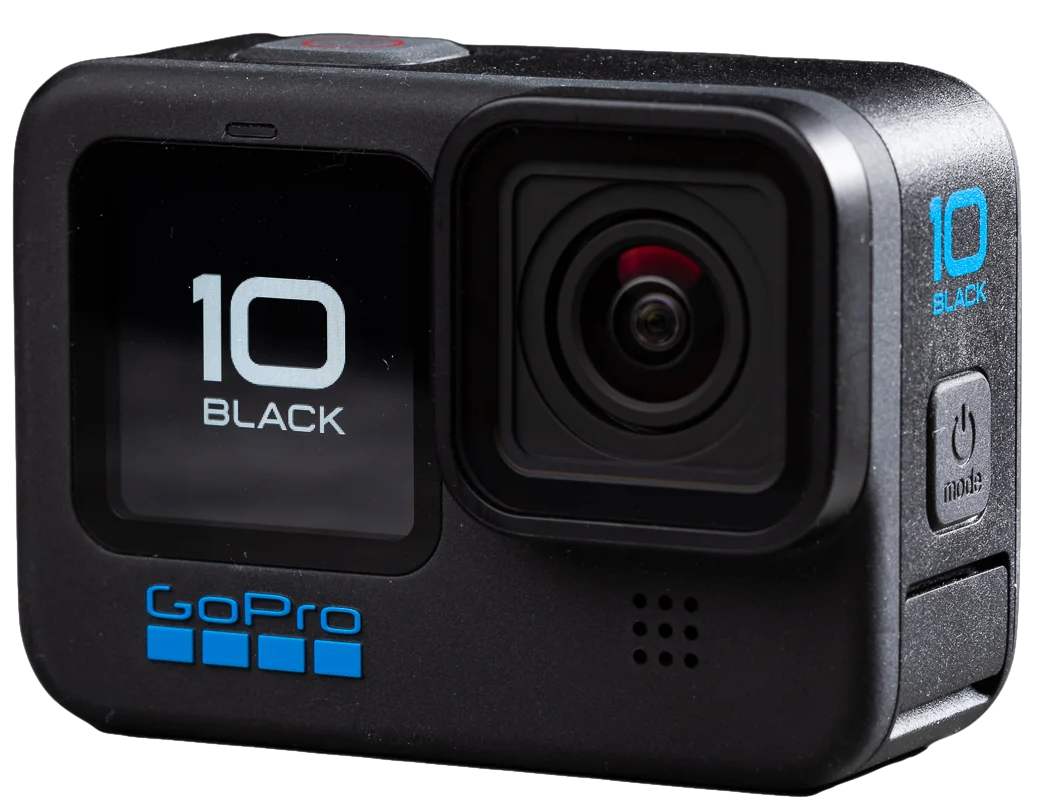
\includegraphics[scale=0.1]{images/fig_chapter1/gopro_hero10.png}
    \caption{GoPro Hero 10}
    \label{fig:gopro_hero10}
\end{figure}


%\begin{itemize}
%\item Why am I doing this?
%\item Why is this relevant?
%\item What concrete problem do we want to solve?
%\item Is this problem big enough?

%\item Why is this exciting?
%\item What makes this problem challenging?
%\item Why an IMU Sensor? Why not just use Images?
%\end{itemize}

%How many times have to captured a video of something and when you looked at it later you found out that the video  is shaky? Image stabilisation is inherent in producing good video quality. Be it a 250,000 Euro television broadcast camera or a 100 euro hobbyist camera, stabilisation of some sort is necessary.


\section{Challenges of the Work}
For this work, an Inertial Measurement Unit (IMU) sensor will be used to stabilise the magnified video. This presents many challenges and requires the use of the state of the art neural network based techniques present today. Some of the challenges that were faced for this work and the requirements are as follows:

\begin{itemize}
\item Sensors are inherent to noise and this especially makes working with an IMU difficult because for position estimation we need to double integrate the signal. This double integration of the noisy signal causes a \textbf{drift} which is very undesirable for any image stabilization algorithm. 
\item Working with this drift is especially not possible in this case as we have a precision requirement of about 0.1 mm for the stabilization to work effectively.
\item There exist IMU sensors with better noise characteristics, however, those are very expensive (in the order of >1000€) and it is difficult to buy them as they usually have a tactical grade placing them under export restrictions. Hence in this work a low-cost consumer MEMS IMU is used.
\item IMUs have been used for position estimation for a long time using the classic Kalman Filter and its variants. They produce acceptable results for some cases but would not work in our case. IMUs are also generally coupled with cameras, GPS and Magnetometers to improve the precision but it is not possible for this use case.
\item  To overcome some of the challenges I am using neural networks. The use of neural networks creates challenges of data generation for training and testing. Neural network implementations for any task require a huge amount of data and the ground truth associated with it.
\item Creating this data is very challenging and a lot of care needs to be taken about domain randomisation so the network generalizes well.
\end{itemize}

There are a lot of challenges in this work to overcome and that makes this exciting. In the next chapter of this report, I will discuss the fundamental of image stabilization and which methods are used.
